%********************************************************************
%***********************ZAŁĄCZNIKI***********************************
%********************************************************************
\titlespacing*{\chapter}{0pt}{-80mm}{40pt} %przesuwanie tytułu rozdziału do góry

\begin{landscape} %strony horyzontalnie
\chapter*{Załączniki}
\addcontentsline{toc}{chapter}{Załączniki}
\vspace{-1cm}
\section*{{\large Załącznik 1. Zmienne wybrane do wstępnej analizy pod kątem zastosowania w~modelu wetorowej autoregresji}}
\vspace{-0.5cm}
\hypertarget{zal1}{}
\begin{table}[h]
\centering
\tiny
\begin{tabular}{|c|c|c|c|c|c|c|llll}
\cline{1-7}
\multirow{2}{*}{\textbf{l.p.}} & \multirow{2}{*}{\textbf{Segment rynku}} & \multirow{2}{*}{\textbf{Nazwa zmiennej}} & \textbf{Nazwa w modelu} & \multirow{2}{*}{\textbf{Jednostka}} & \textbf{Stopień}  & \multirow{2}{*}{\textbf{Źródło}} &  &  &  &  \\ 
 &  &  & \textbf{VAR} & & \textbf{zintegrowania} &  &  &  &  &  \\
\cline{1-7}
1. & \multirow{5}{*}{Poziom cen} & Indeks prywatnych wydatków konsumpcyjnych & PCE & Roczna zmiana (w \%) & 0 & \url{https://fred.stlouisfed.org/series/PCE} &  &  &  &  \\ \cline{1-1} \cline{3-7}
2.            &                                                  & Index cen dóbr produkcyjnych & PPI                              & Roczna zmiana (w \%) & 0 & \url{https://fred.stlouisfed.org/series/PPIACO}            &  &  &  &  \\ \cline{1-1} \cline{3-7}
3.            &                                                  & 
Baza monetarna & Baza\_mon                        & Miliony dolarów &  1   & \url{https://fred.stlouisfed.org/series/MBCURRCIR\#0}      &  &  &  &  \\ \cline{1-1} \cline{3-7}
4.   &                                    & Oczekiwania inflacyjne & InflExp                          & Punkty procentowe    & 0 & \url{https://fred.stlouisfed.org/series/MICH}             &  &  &  & \\ \cline{1-1} \cline{3-7} 
5.           &  &  Wartość papierów wartościowych w bilansie Rezerwy Federalnej                                 & FED\_Securities                  & Miliony dolarów      & 1 & \url{https://fred.stlouisfed.org/series/WSHOL}            &  &  &  &  \\ \cline{1-7}
6.            & \multirow{3}{*}{Rynek pracy}                     & Stopa bezrobocia & Stopa\_bez                       & Punkty procentowe  & 2  & \url{https://fred.stlouisfed.org/series/UNRATE}          &  &  &  &  \\ \cline{1-1} \cline{3-7}
7.            &                                                  & Poziom zatrudnienia pozarolniczego & Zatrudnienie                     & Tysiące osób     & 2  & \url{https://fred.stlouisfed.org/series/PAYEMS}            &  &  &  &  \\ \cline{1-1} \cline{3-7}
8.            &                                                  & Mediana czasu trwania bezrobocia                                                            & UnempDur                         & Tygodnie             & 1 & \url{https://fred.stlouisfed.org/series/LNU03008276}      &  &  &  &  \\ \cline{1-7}
9.            & \multirow{2}{*}{Poziom produkcji}                & Roczna zmiana PKB realnego & PKB\_realne                      & Punkty procentowe & 1 & \url{http://www.macroadvisers.com/monthly-gdp}            &  &  &  &  \\ \cline{1-1} \cline{3-7}
10.            &                                                  & Indeks Produkcji Przemysłowej & IPP                              & Punkty indeksowe &  1  & \url{https://fred.stlouisfed.org/series/INDPRO}           &  &  &  &  \\ \cline{1-7}
11.           & \multirow{3}{*}{Rynek obligacji skarbowych}      & Rentowność rocznych obligacji skarbowych & Yield1YGov                       & Punkty procentowe  & 2  & \url{https://fred.stlouisfed.org/series/DGS1}              &  &  &  &  \\ \cline{1-1} \cline{3-7}
12.           &                                                  & Rentowność dziesięcioletnich obligacji skarbowych & Yield10Gov                       & Punkty procentowe  & 1  & \url{https://fred.stlouisfed.org/series/DGS10}             &  &  &  &  \\ \cline{1-1} \cline{3-7}
13.           &                                                  & Spread pomiędzy rentownością dziesięcioletnich i dwuletnich obligacji                 & Spread2Y10Y                      & Punkty procentowe  & 1 & \url{https://fred.stlouisfed.org/series/T10Y2Y\#0}        &  &  &  &  \\ \cline{1-7}
14.           & \multirow{3}{*}{Rynek obligacji korporacyjnych}  & Rentowność obligacji korporacyjnych z ratingiem AAA & CorpAAAYields                    & Punkty procentowe    & 1 & \url{https://fred.stlouisfed.org/series/BAMLC0A1CAAAEY\#0} &  &  &  &  \\ \cline{1-1} \cline{3-7}
15.           &                                                  & Rentowność obligacji korporacyjnych z ratingiem BBB                                        & CorpBBBYields                    & Punkty procentowe    &  1 & \url{https://fred.stlouisfed.org/series/BAMLC0A4CBBBEY}    &  &  &  &  \\ \cline{1-1} \cline{3-7}
16.           &                                                  & Rentowność obligacji korporacyjnych z ratingiem CCC                              & CorpCCCYields                    & Punkty procentowe    & 1  & \url{https://fred.stlouisfed.org/series/BAMLH0A3HYCEY\#0}  &  &  &  &  \\ \cline{1-7}
17.           & \multirow{2}{*}{Rynek międzybankowy}             & Efektywna Stopa Funduszy Federalnych & EFFR                             & Punkty procentowe    &  0   & \url{https://fred.stlouisfed.org/series/EXUSUK}           &  &  &  &  \\ \cline{1-1} \cline{3-7}
18.           &                                                  & TED spread                                                                                 & TED\_spread                      & Punkty procentowe    &  1   & \url{https://fred.stlouisfed.org/series/TEDRATE}         &  &  &  &  \\ \cline{1-7}
19.           & \multirow{3}{*}{Stopy wolne od ryzyka}           & Trzydziestoletnia stopa swap                                                                          & Swap30Year                       & Punkty procentowe    &  1 & \url{https://fred.stlouisfed.org/series/DSWP30}           &  &  &  &  \\ \cline{1-1} \cline{3-7}
20.           &                                                  & Dziesięcioletnia stopa swap                                                                          & Swap10Year                       & Punkty procentowe    &  1  & \url{https://fred.stlouisfed.org/series/DSWP10}           &  &  &  &  \\ \cline{1-1} \cline{3-7}
21.           &                                                  & Roczna stopa swap & Swap1Year                        & Punkty procentowe  & 2  & \url{https://fred.stlouisfed.org/series/DSWP1}             &  &  &  &  \\ \cline{1-7}
22.           & \multirow{5}{*}{Rynek walutowy}                  & Indeks wartości dolara ważony handlem & USD\_Trade                       & Roczna zmiana (w \%) & 1 & \url{https://fred.stlouisfed.org/series/TWEXB}             &  &  &  &  \\ \cline{1-1} \cline{3-7}
23.           &                                                  & Kurs walutowy EUR/USD & EURUSD                           & Kurs walutowy  &  1  & \url{https://fred.stlouisfed.org/series/EXUSEU}           &  &  &  &  \\ \cline{1-1} \cline{3-7}
24.           &                                                  & Kurs walutowy GPB/USD  & GBPUSD                           & Kurs walutowy    &  0 & \url{https://fred.stlouisfed.org/series/EXUSUK}           &  &  &  &  \\ \cline{1-1} \cline{3-7}
25.           &                                                  & Kurs walutowy USD/JPY  & USDJPY                           & Kurs walutowy   & 1 & \url{https://fred.stlouisfed.org/series/EXJPUS}            &  &  &  &  \\ \cline{1-1} \cline{3-7}
26.           &                                                  & Kurs walutowy USD/CNY & USDCNY                           & Kurs walutowy   & 2  & \url{https://fred.stlouisfed.org/series/EXCHUS}            &  &  &  &  \\ \cline{1-7}
27.           & Rynek akcji                                      & Indeks S\&P500                                                                                    & SP500                            & Punkty indeksowe     & 1 & \url{https://fred.stlouisfed.org/series/SP500}           &  &  &  &  \\ \cline{1-7}
28.           & Rynek nieruchomości                              & Indeks cen domów & House\_Price                     & Punkty indeksowe   & 1 & \url{https://fred.stlouisfed.org/series/HPIPONM226S}       &  &  &  &  \\ \cline{1-7}
29.           & Rynek instrumentów pochodnych                    & Indeks VIX & VIX                              & Punkty indeksowe     & 1 & \url{https://fred.stlouisfed.org/series/VIXCLS\#0}        &  &  &  &  \\ \cline{1-7}
30.           & Rynek kredytów bankowych                         & Wartość kredytów udzielonych przez banki komercyjne & Kred\_bank                       & Miliony dolarów  &  2  & \url{https://fred.stlouisfed.org/series/TOTBKCR}           &  &  &  &  \\ \cline{1-7}
31.           & Poziom konsumpcji                                &  Wydatki konsumpcyjne                                  & Pers\_cons                       & Punkty indeksowe  & 1   & \url{https://fred.stlouisfed.org/series/PCEPI}           &  &  &  &  \\ \cline{1-7}
32.           & Rynek surowcowy                                  & Cena złota & Gold\_Price                      & Dolary za uncje      & 1 & \url{https://fred.stlouisfed.org/series/GOLDAMGBD228NLBM}  &  &  &  &  \\ \cline{1-7}
\end{tabular}
\begin{flushleft}
 \textit{\tiny{Źródło: Opracowanie własne.}} \\
\end{flushleft}
\end{table}

\end{landscape}

\newpage
\hypertarget{zal2}{}
\section*{{\large Załącznik 2. Diagramy dopasowań oraz reszt zmiennych w~modelu VAR}}

\hypertarget{fig100}{}
\begin{figure}[H]
\begin{subfigure}{.5\textwidth}
\caption{Indeks prywatnych wydatków konsumpcyjnych}
\hspace{-3cm}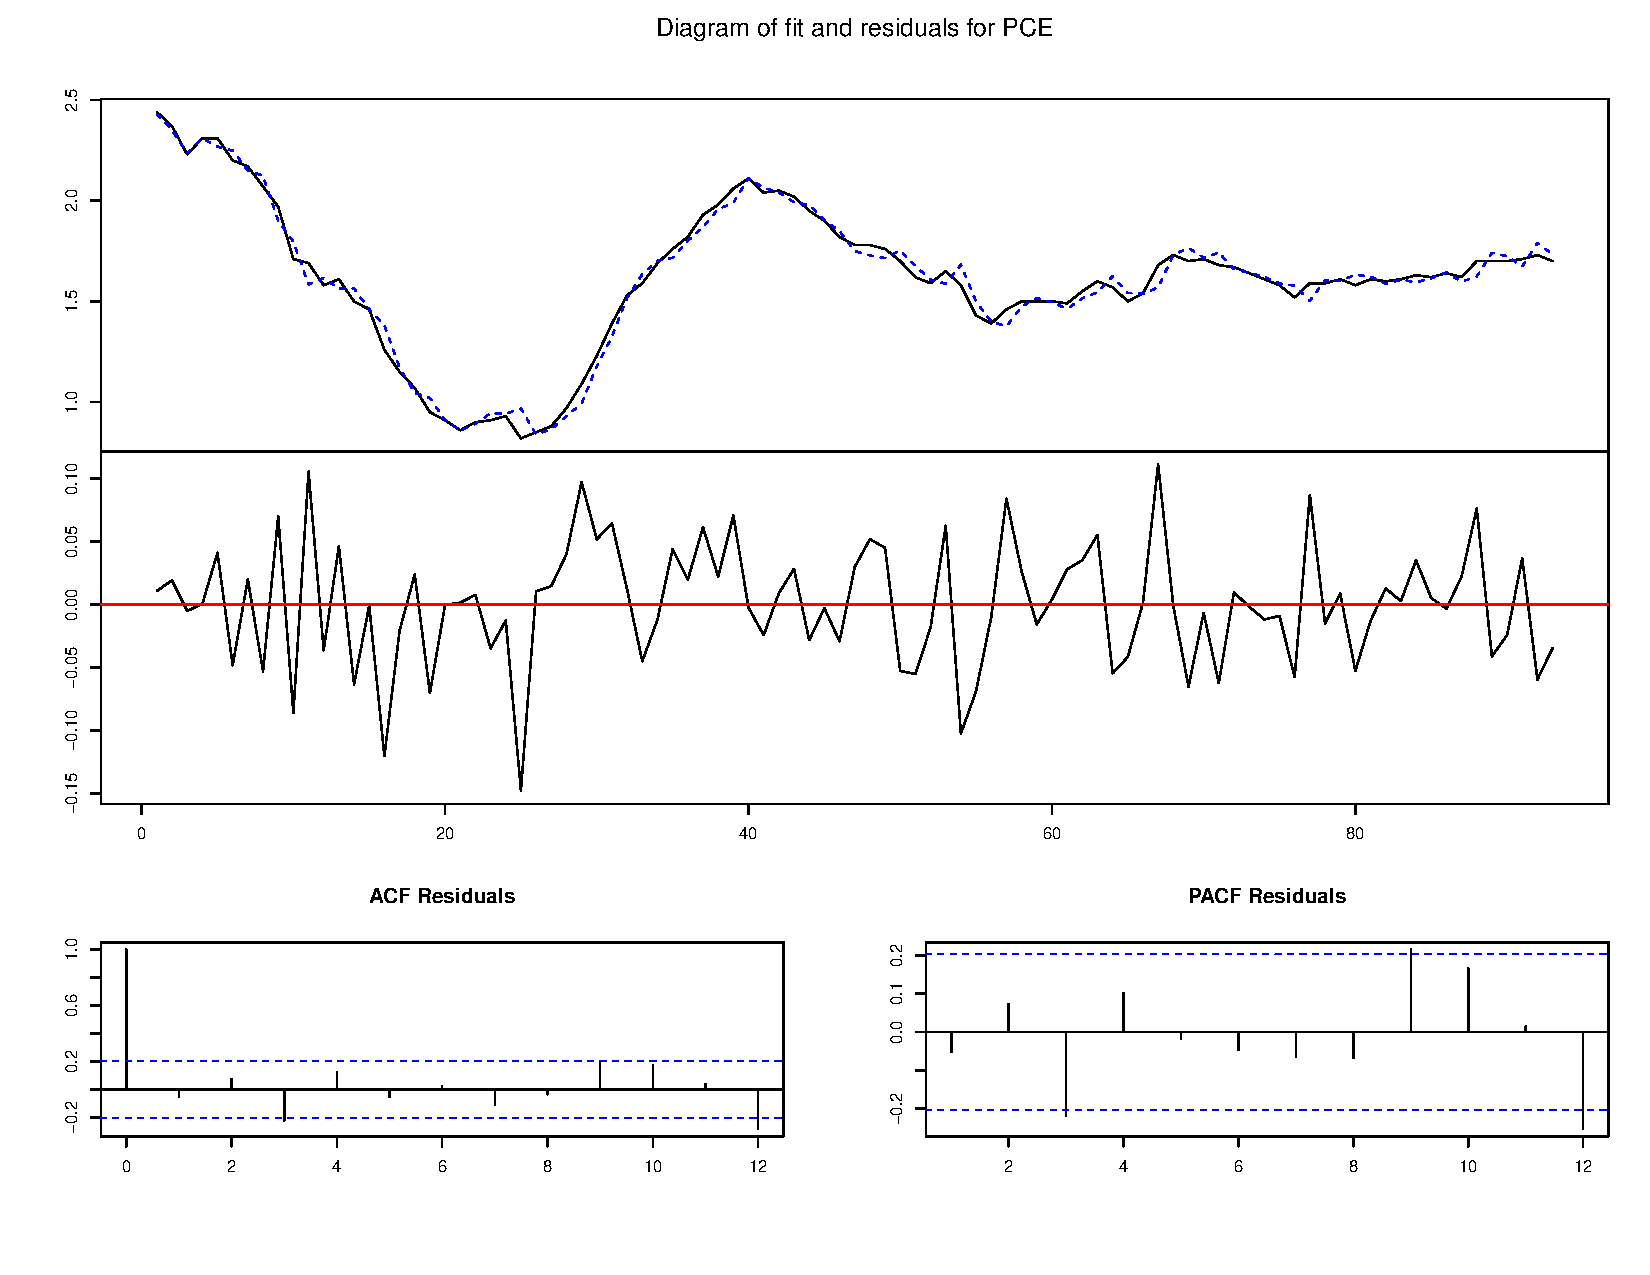
\includegraphics[height=4in]{PCE}
\end{subfigure}
\vspace{-0.75cm}
\begin{flushleft}
\hspace{1cm}\textit{\footnotesize{Źródło: Opracowanie własne.}} \\
\end{flushleft}
\end{figure}

\vspace{-1cm}

\hypertarget{fig101}{}
\begin{figure}[H]
\ContinuedFloat
\centering
\begin{subfigure}{.5\textwidth}
\caption{Stopa bezrobocia}
\hspace{-3cm}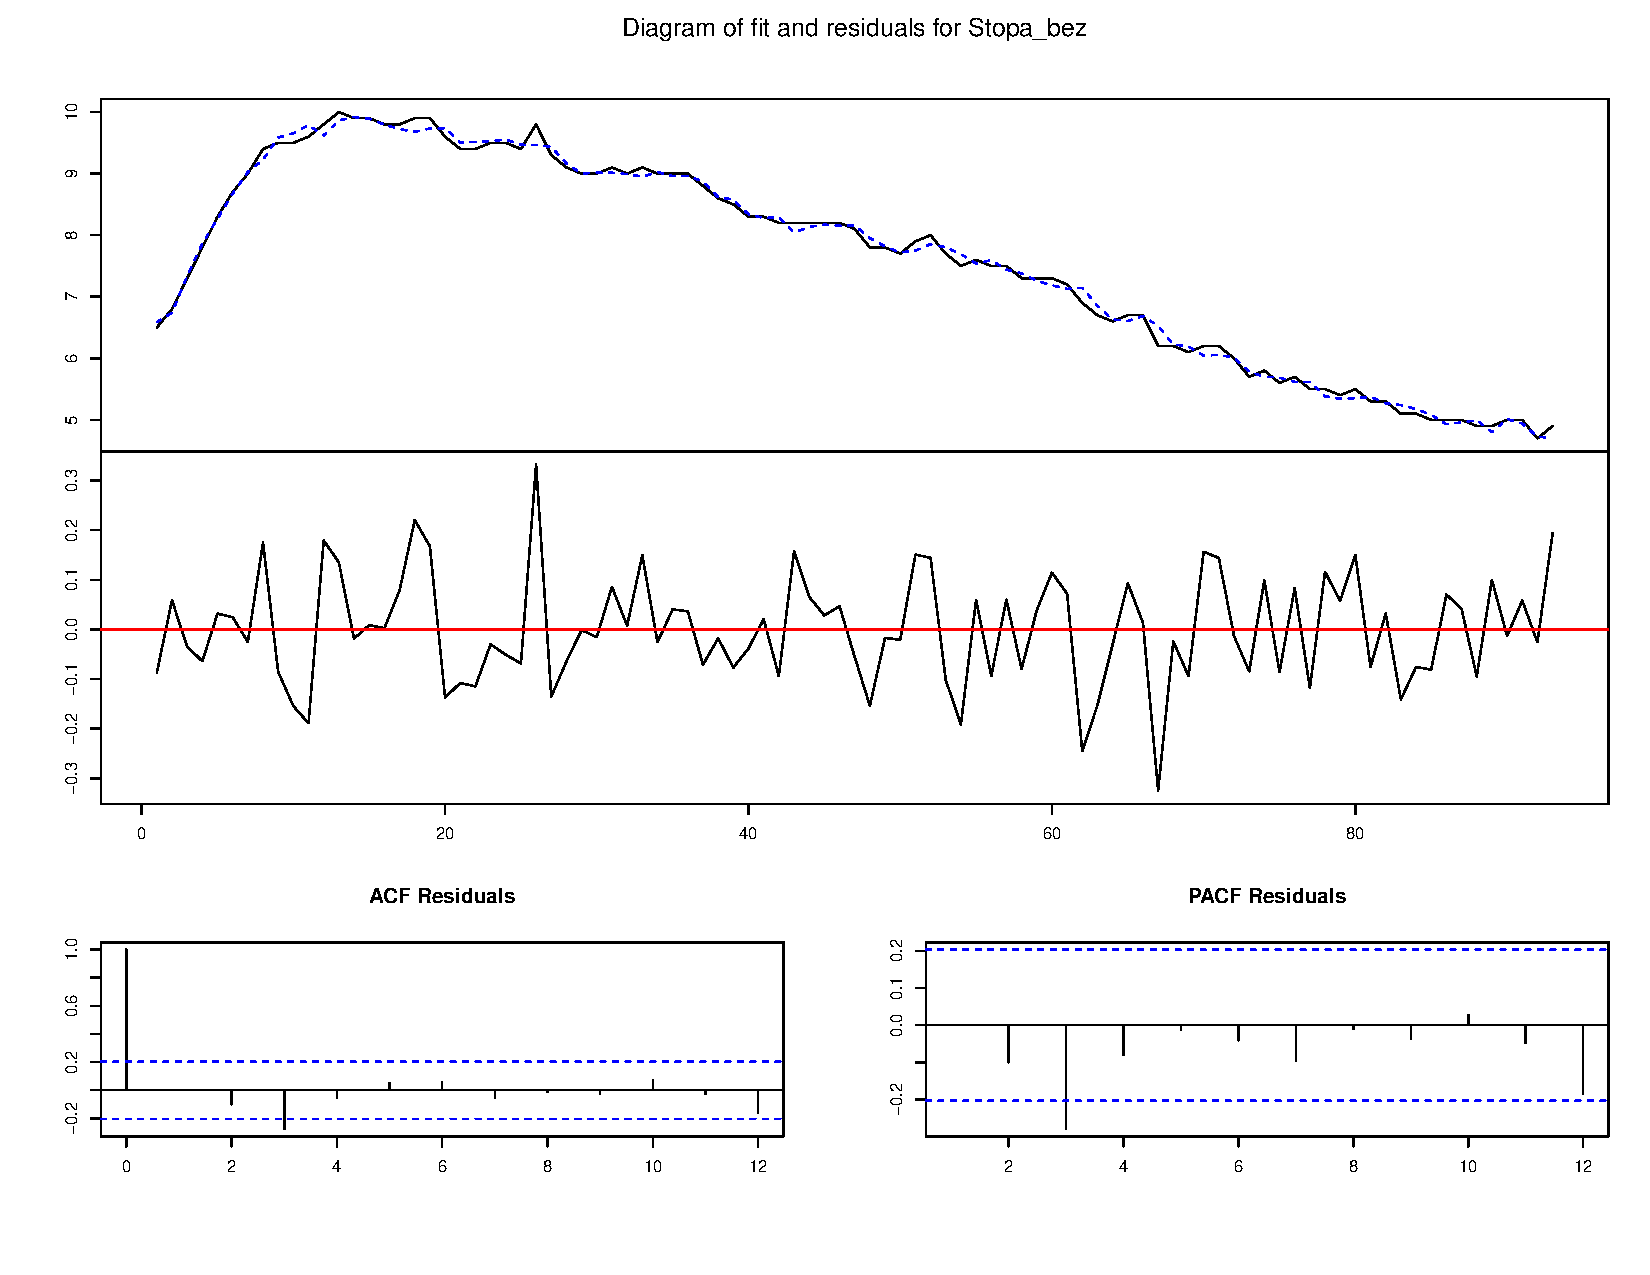
\includegraphics[height=4in]{StopaBez}
\end{subfigure}
\vspace{-0.75cm}
\begin{flushleft}
\hspace{1cm}\textit{\footnotesize{Źródło: Opracowanie własne.}} \\
\end{flushleft}
\end{figure}

\vspace{-1cm}

\hypertarget{fig102}{}
\begin{figure}[H]
\ContinuedFloat
\centering
\begin{subfigure}{.5\textwidth}
\caption{Roczna zmiana PKB realnego}
\hspace{-3cm}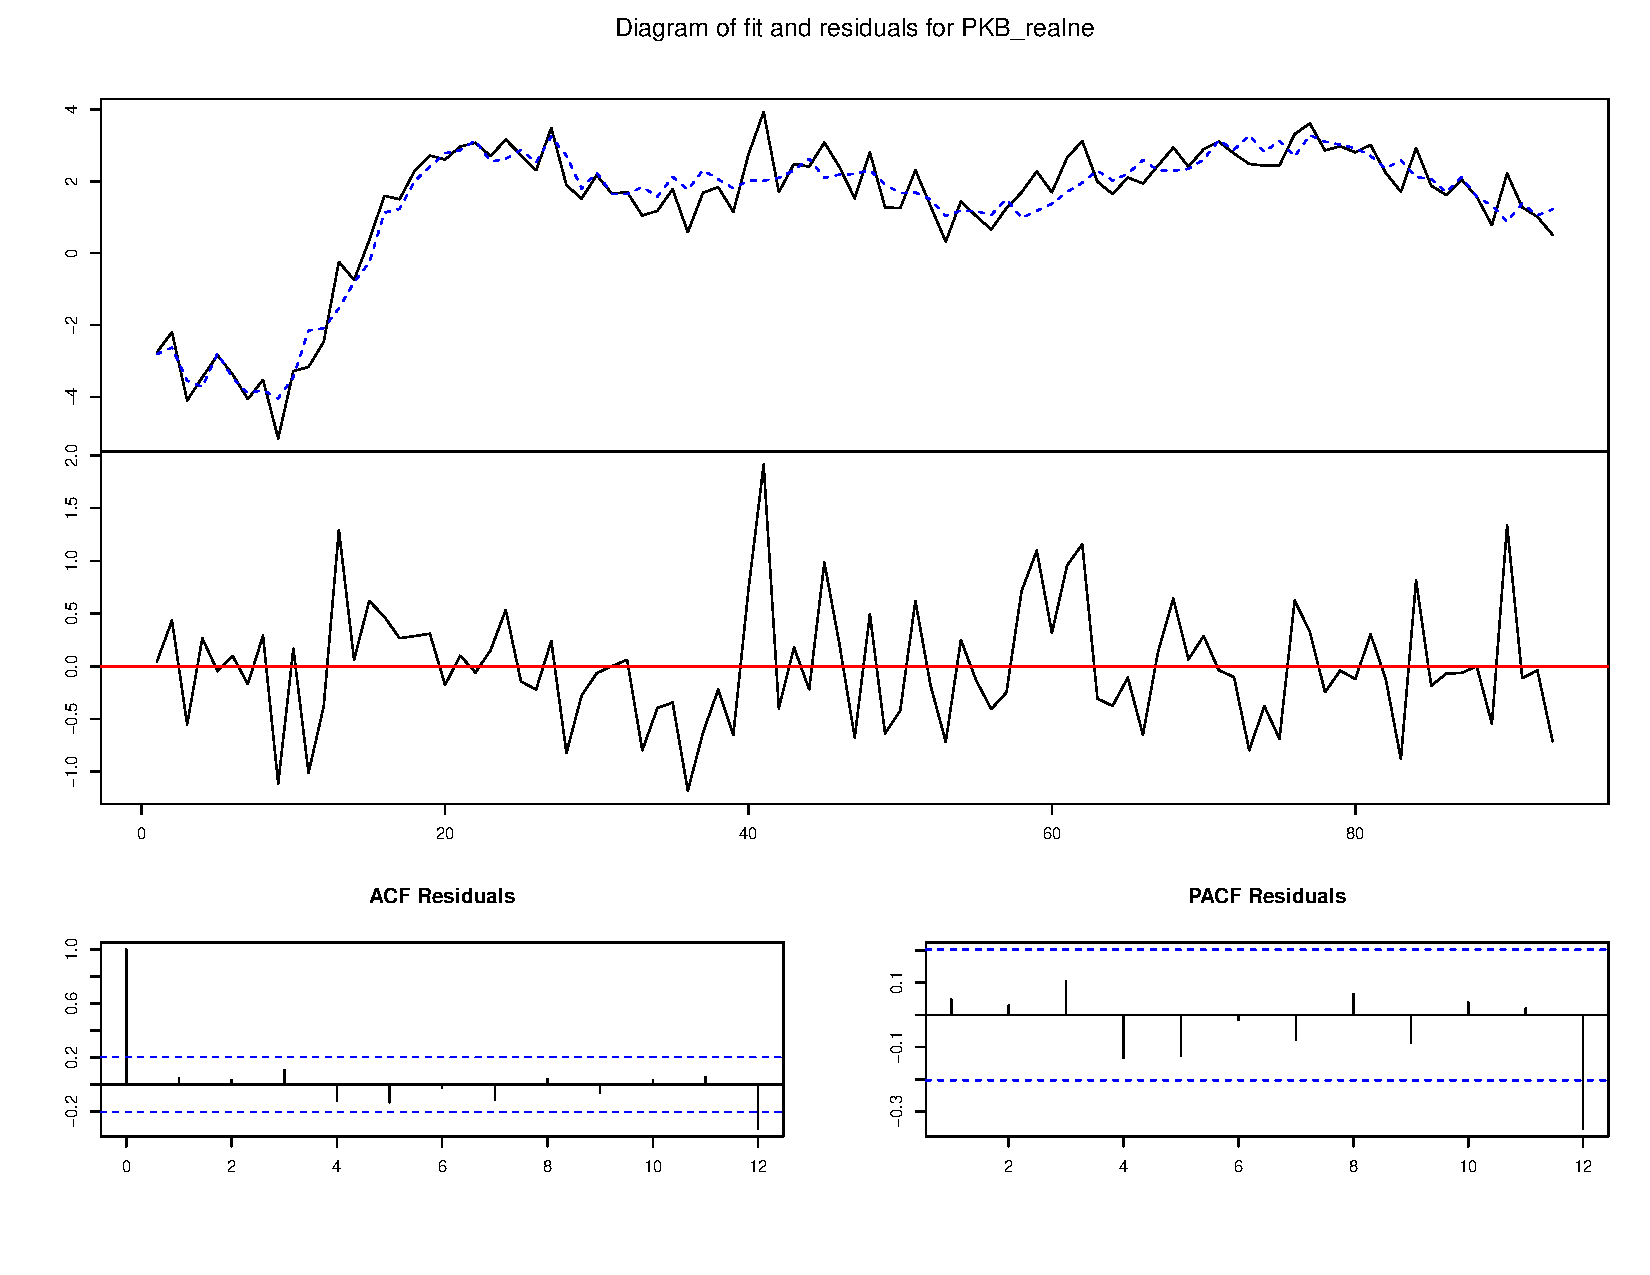
\includegraphics[height=4in]{PKB}
\end{subfigure}
\vspace{-0.75cm}
\begin{flushleft}
\hspace{1cm}\textit{\footnotesize{Źródło: Opracowanie własne.}} \\
\end{flushleft}
\end{figure}

\vspace{-1cm}

\hypertarget{fig103}{}
\begin{figure}[H]
\ContinuedFloat
\centering
\begin{subfigure}{.5\textwidth}
\caption{Indeks S\&P500}
\hspace{-3cm}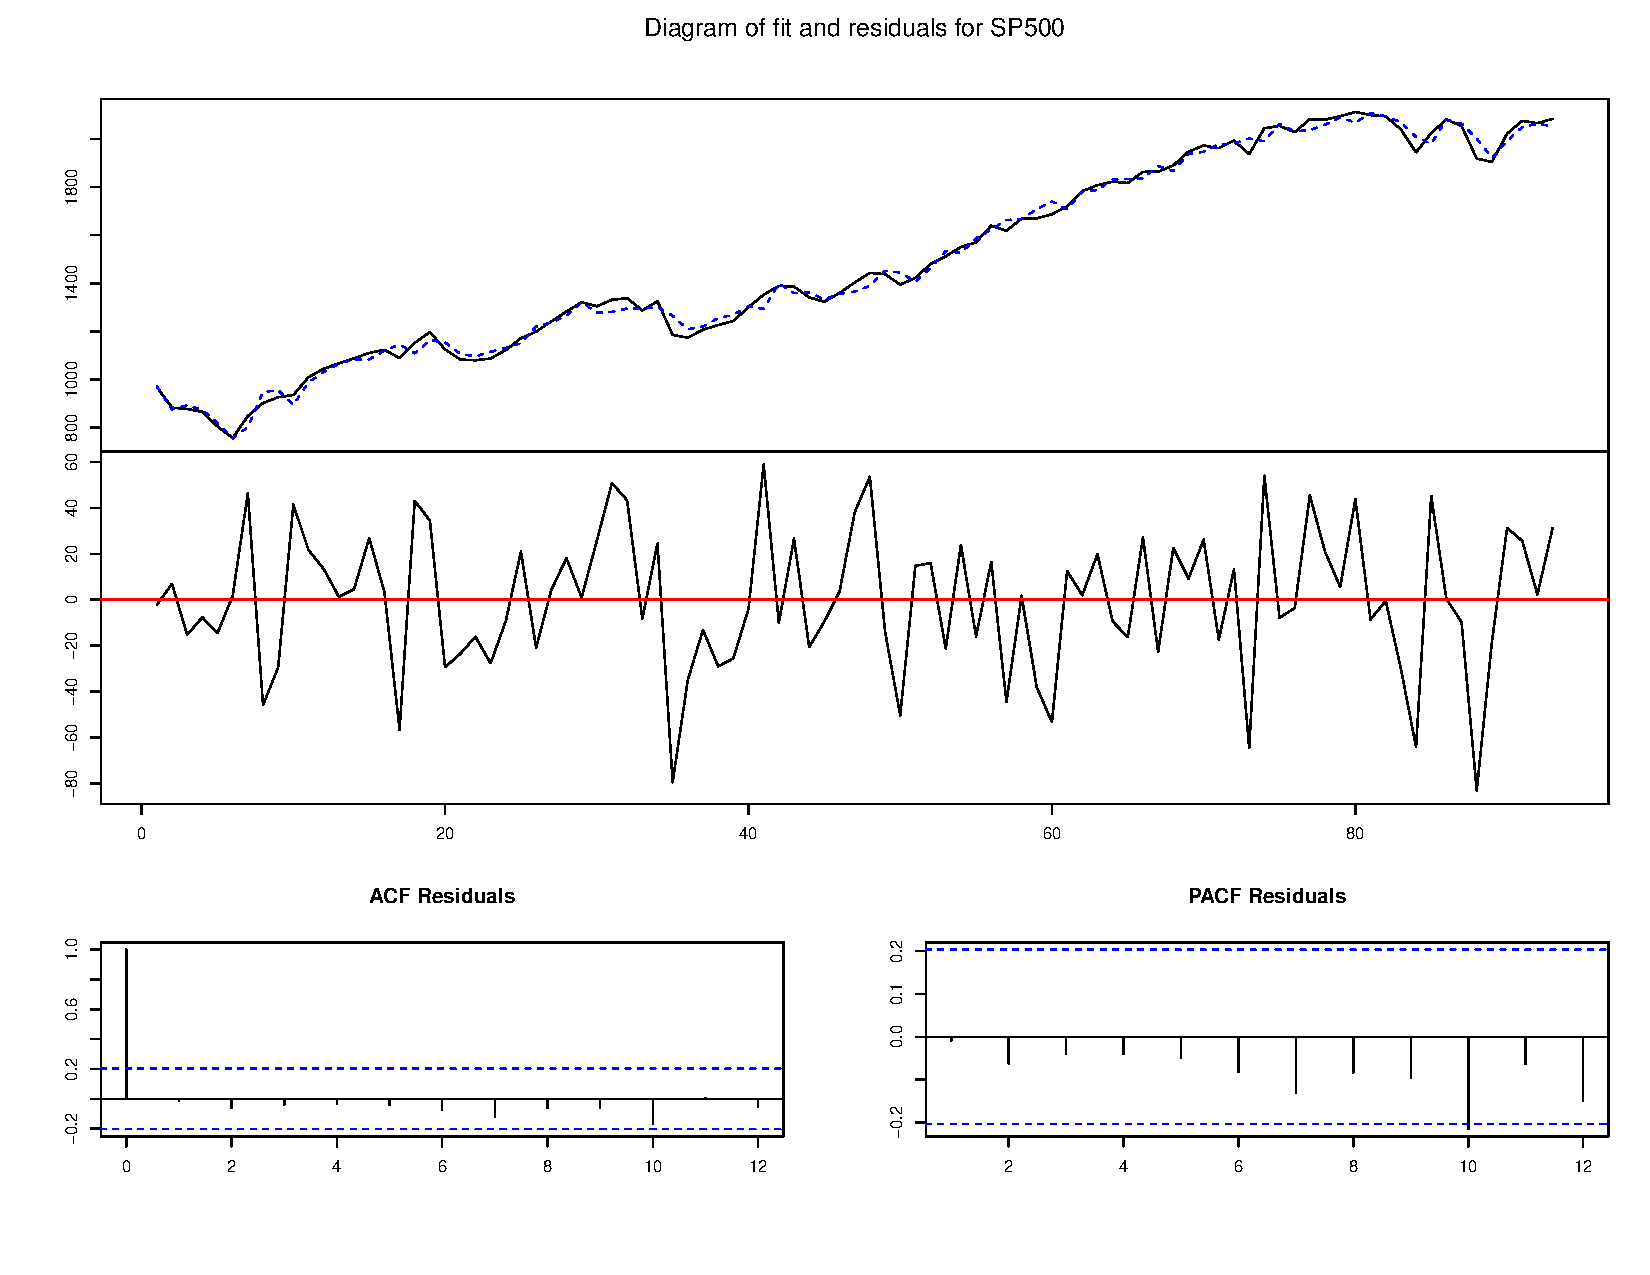
\includegraphics[height=4in]{SP500}
\end{subfigure}
\vspace{-0.75cm}
\begin{flushleft}
\hspace{1cm}\textit{\footnotesize{Źródło: Opracowanie własne.}} \\
\end{flushleft}
\end{figure}

\vspace{-1cm}

\hypertarget{fig104}{}
\begin{figure}[H]
\ContinuedFloat
\centering
\begin{subfigure}{.5\textwidth}
\caption{Rentowność rocznych obligacji skarbowych}
\hspace{-3cm}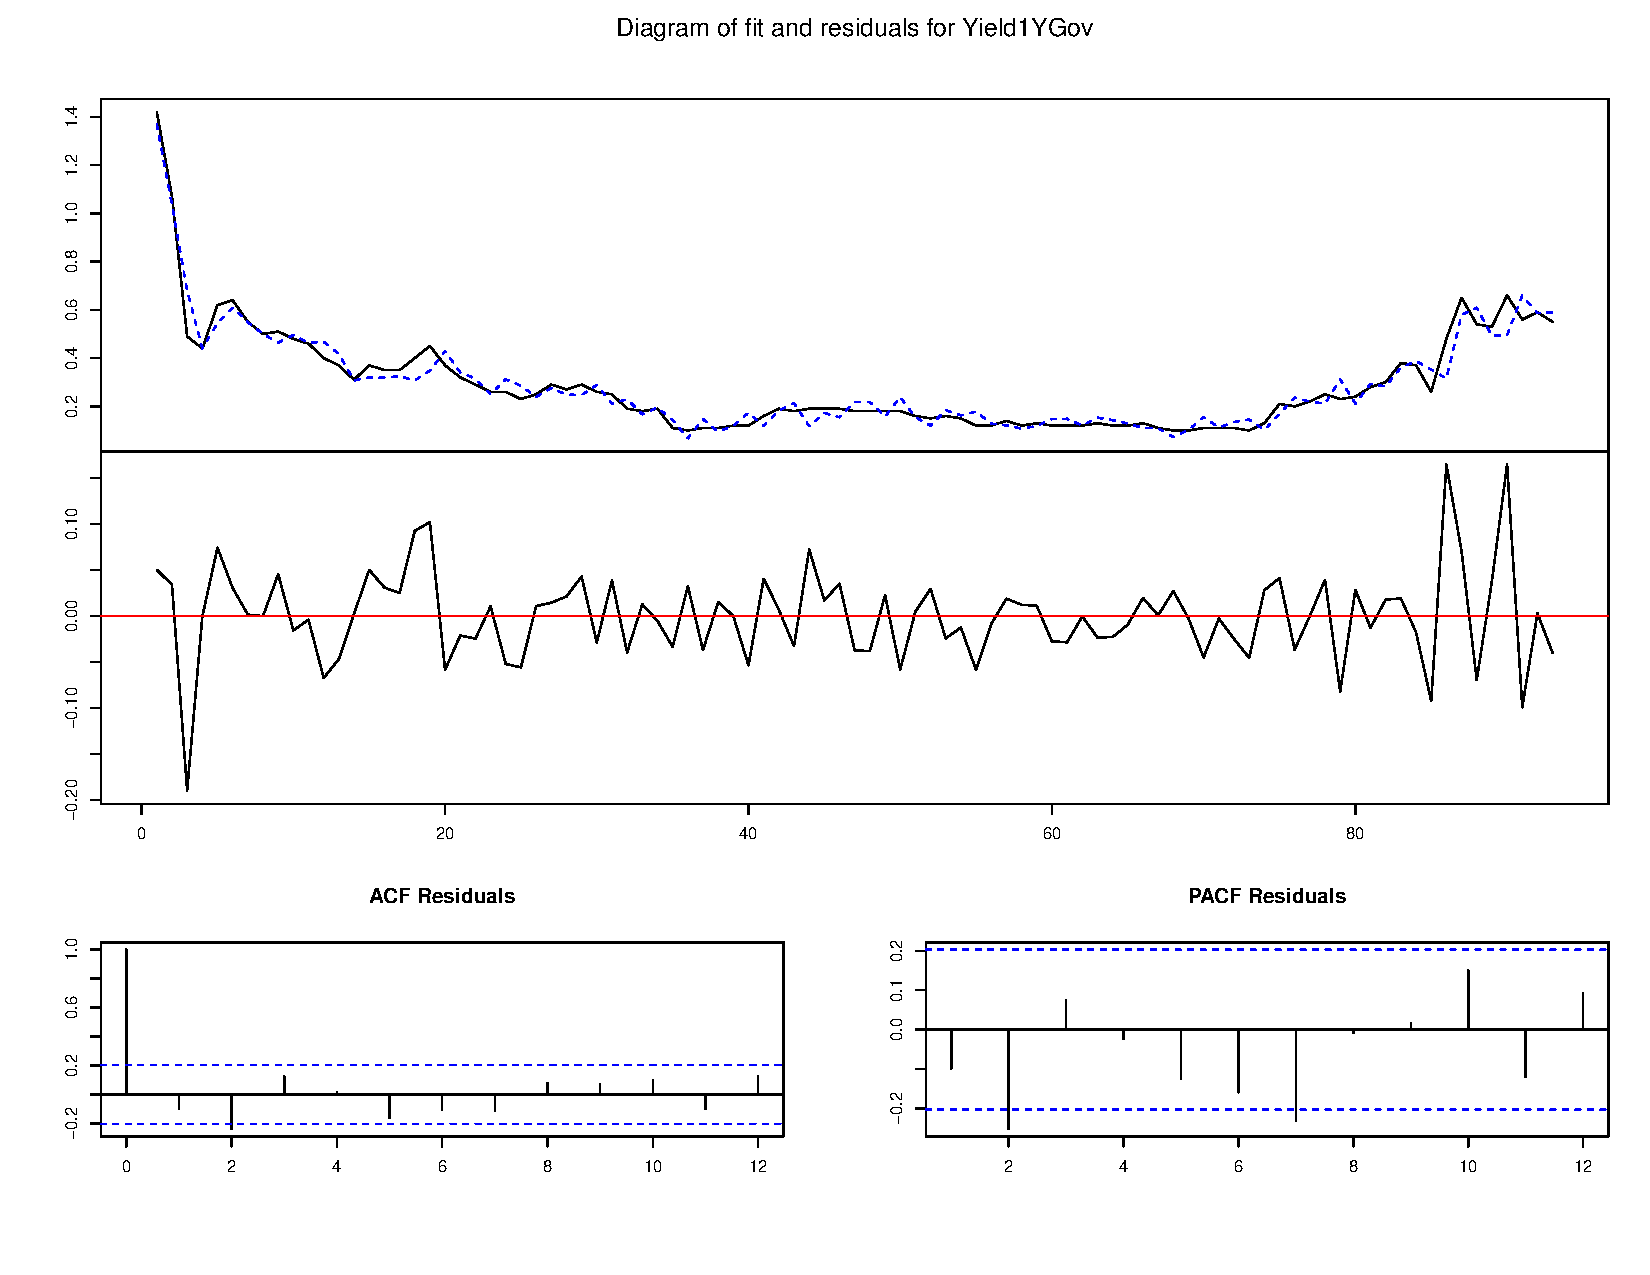
\includegraphics[height=4in]{Yield1}
\end{subfigure}
\vspace{-0.75cm}
\begin{flushleft}
\hspace{1cm}\textit{\footnotesize{Źródło: Opracowanie własne.}} \\
\end{flushleft}
\end{figure}

\vspace{-1cm}

\hypertarget{fig105}{}
\begin{figure}[H]
\ContinuedFloat
\centering
\begin{subfigure}{.5\textwidth}
\caption{Rentowność 10-letnich obligacji skarbowych}
\hspace{-3cm}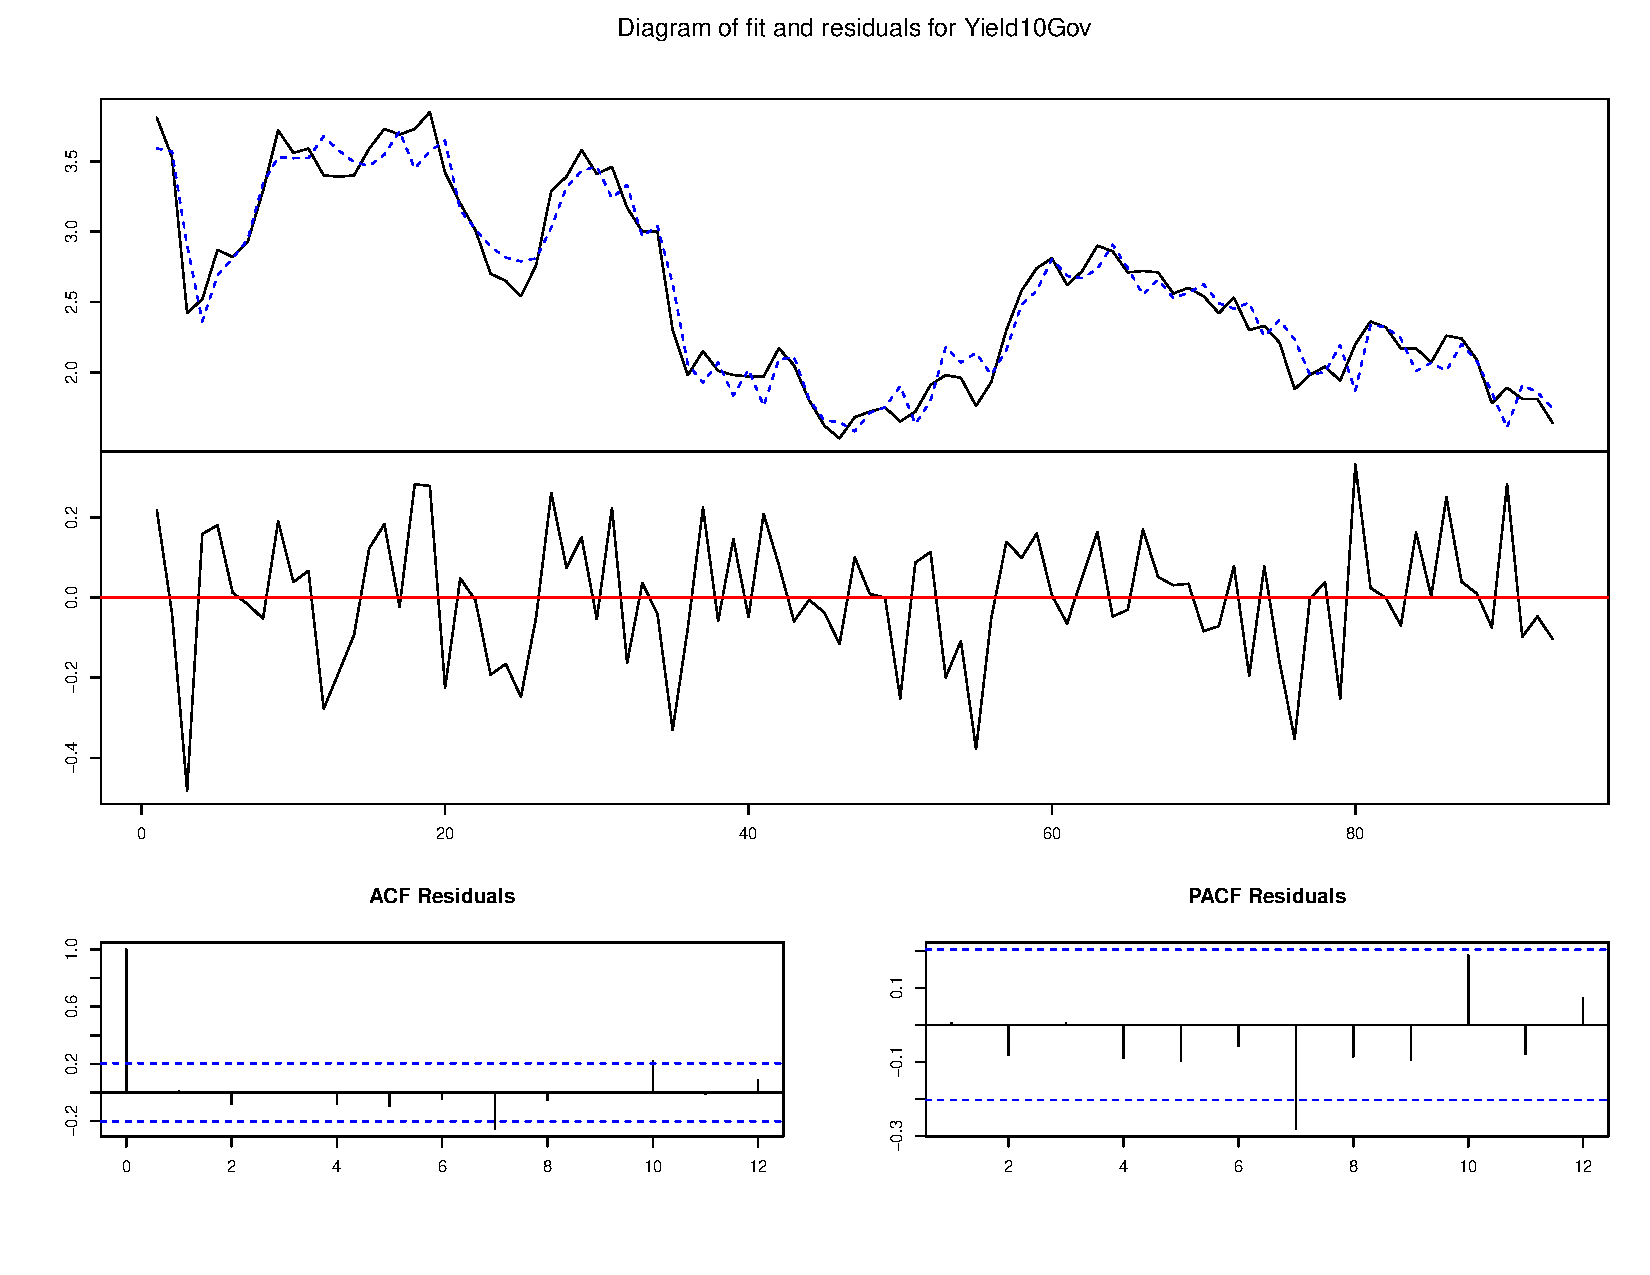
\includegraphics[height=4in]{Yield10}
\end{subfigure}
\vspace{-0.75cm}
\begin{flushleft}
\hspace{1cm}\textit{\footnotesize{Źródło: Opracowanie własne.}} \\
\end{flushleft}
\end{figure}

\vspace{-1cm}

\hypertarget{fig106}{}
\begin{figure}[H]
\ContinuedFloat
\centering
\begin{subfigure}{.5\textwidth}
\caption{Wartość papierów wartościowych FED}
\hspace{-3cm}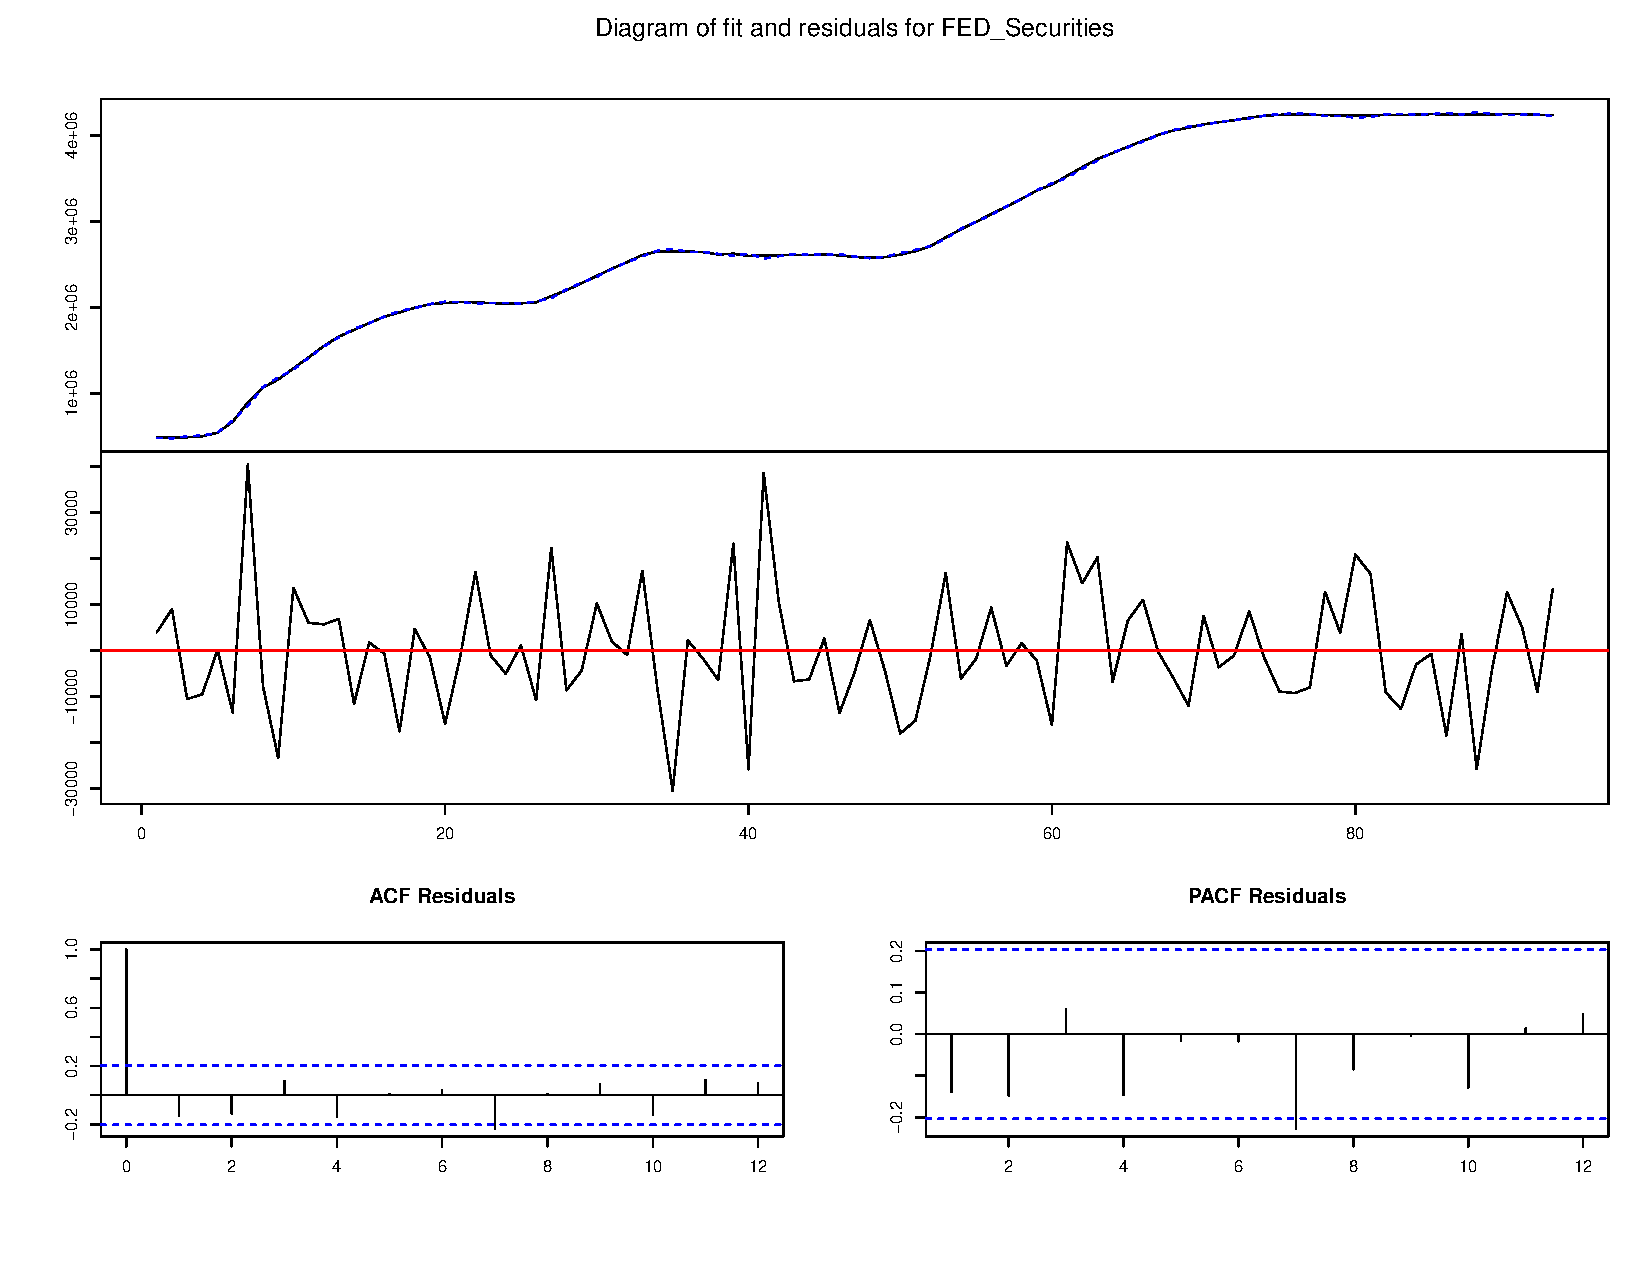
\includegraphics[height=4in]{FED}
\end{subfigure}
\vspace{-0.75cm}
\begin{flushleft}
\hspace{1cm}\textit{\footnotesize{Źródło: Opracowanie własne.}} \\
\end{flushleft}
\end{figure}

\vspace{-1cm}

\hypertarget{fig107}{}
\begin{figure}[H]
\ContinuedFloat
\centering
\begin{subfigure}{.5\textwidth}
\caption{Mediana czasu trwania bezrobocia}
\hspace{-3cm}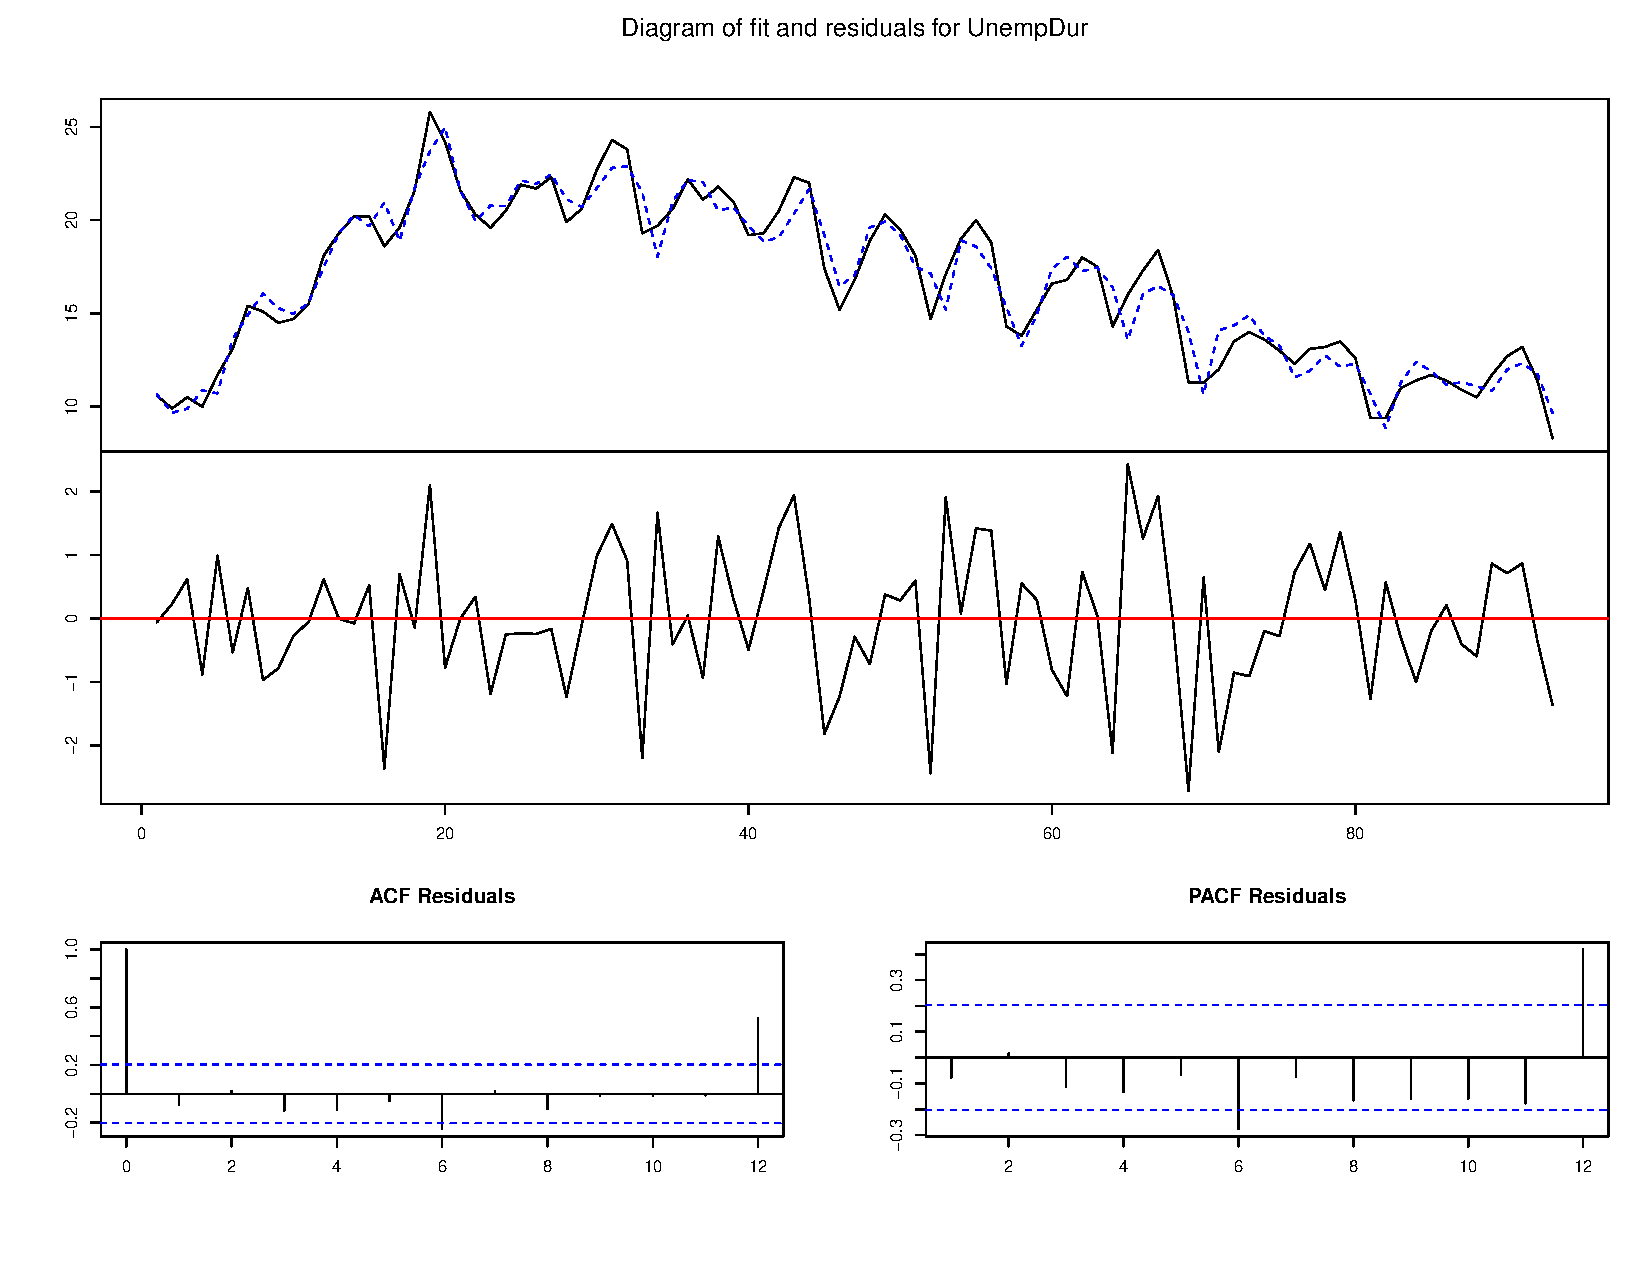
\includegraphics[height=4in]{Unemp}
\end{subfigure}
\vspace{-0.75cm}
\begin{flushleft}
\hspace{1cm}\textit{\footnotesize{Źródło: Opracowanie własne.}} \\
\end{flushleft}
\end{figure}

\vspace{-1cm}

\hypertarget{fig108}{}
\begin{figure}[H]
\ContinuedFloat
\centering
\begin{subfigure}{.5\textwidth}
\caption{Kurs walutowy EUR/USD}
\hspace{-3cm}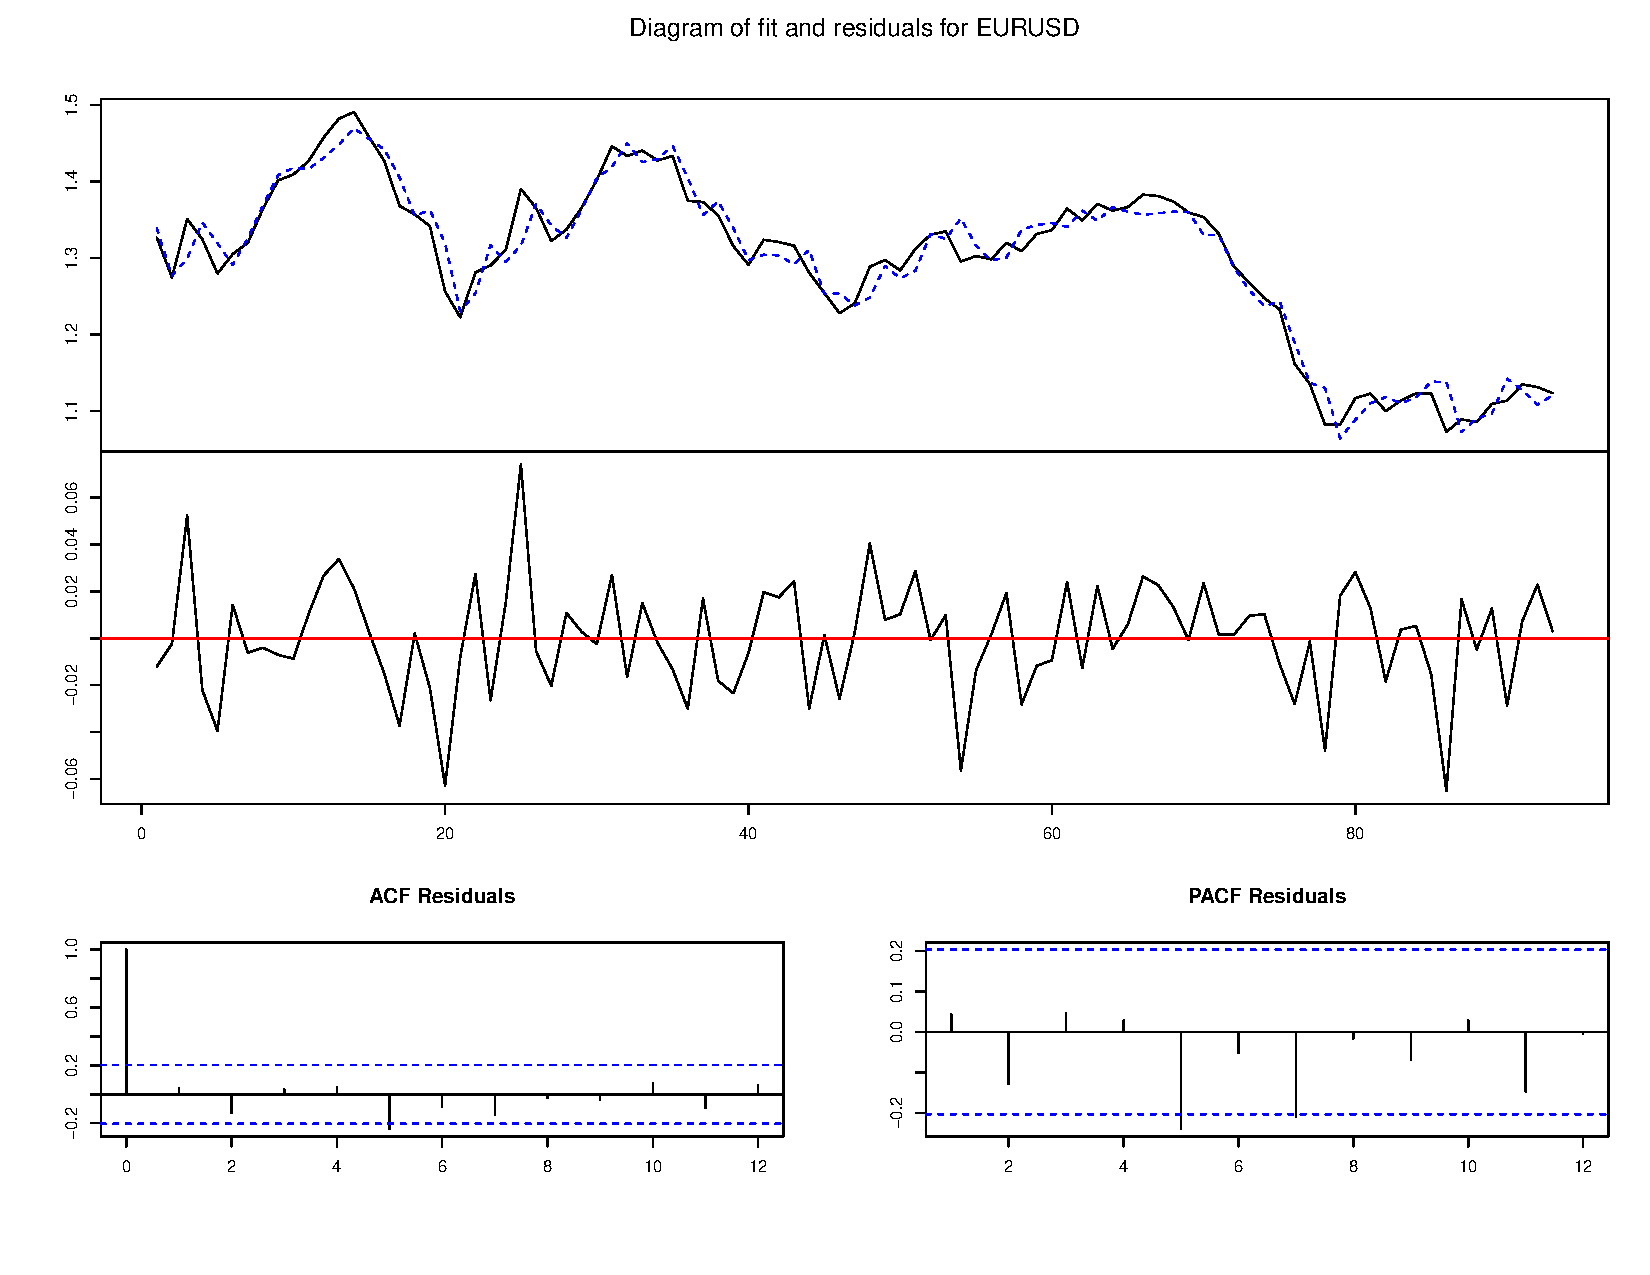
\includegraphics[height=4in]{EURUSD}
\end{subfigure}
\vspace{-0.75cm}
\begin{flushleft}
\hspace{1cm}\textit{\footnotesize{Źródło: Opracowanie własne.}} \\
\end{flushleft}
\end{figure}
